\chapter{Joint Beamforming Design for RIS-aided DFRC system}\label{cha:joint-design}
In this section, the detailed design of joint active and passive beamforming for DFRC system is exposed, where the 
WSR and probing power at target are maximized simultaneously.

% \begin{figure}[htbp]
%   \centering
%   \subfigure[Separated Deployment]{
%       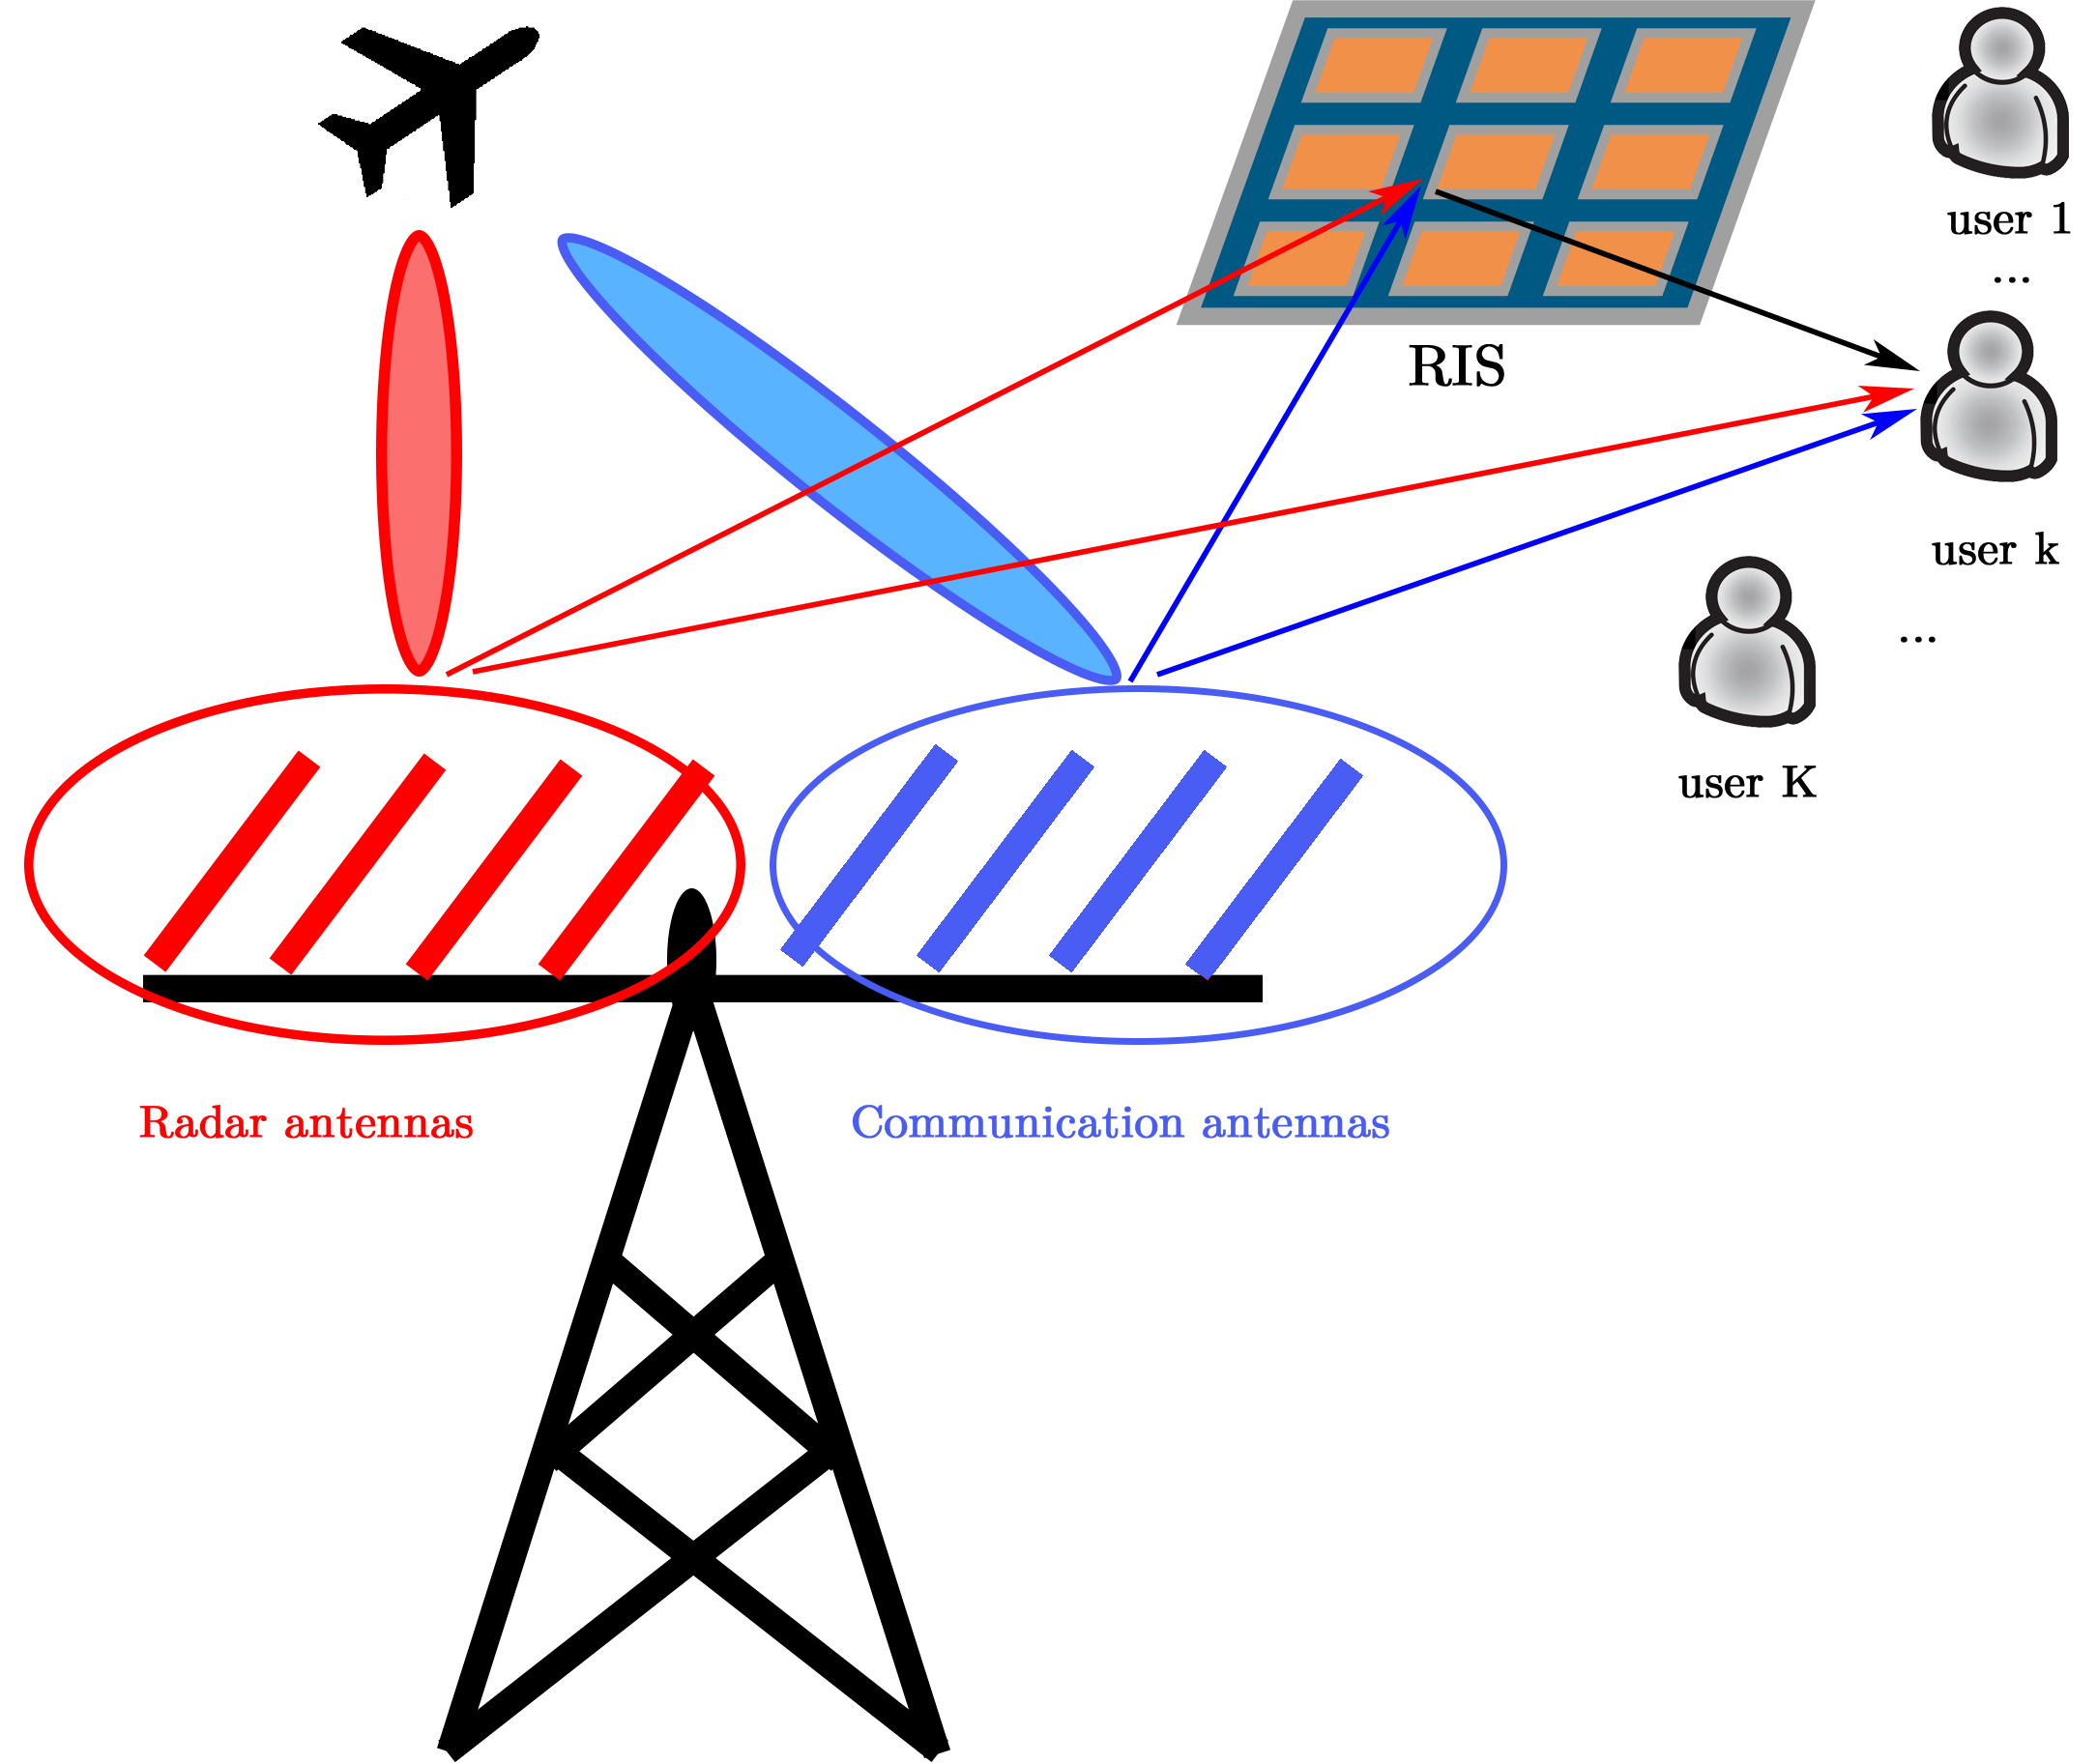
\includegraphics[width=0.42\textwidth]{./separated_setup.png}
%       \label{fig:setup_separated}
%   }
%   \subfigure[Shared Deployment]{
% 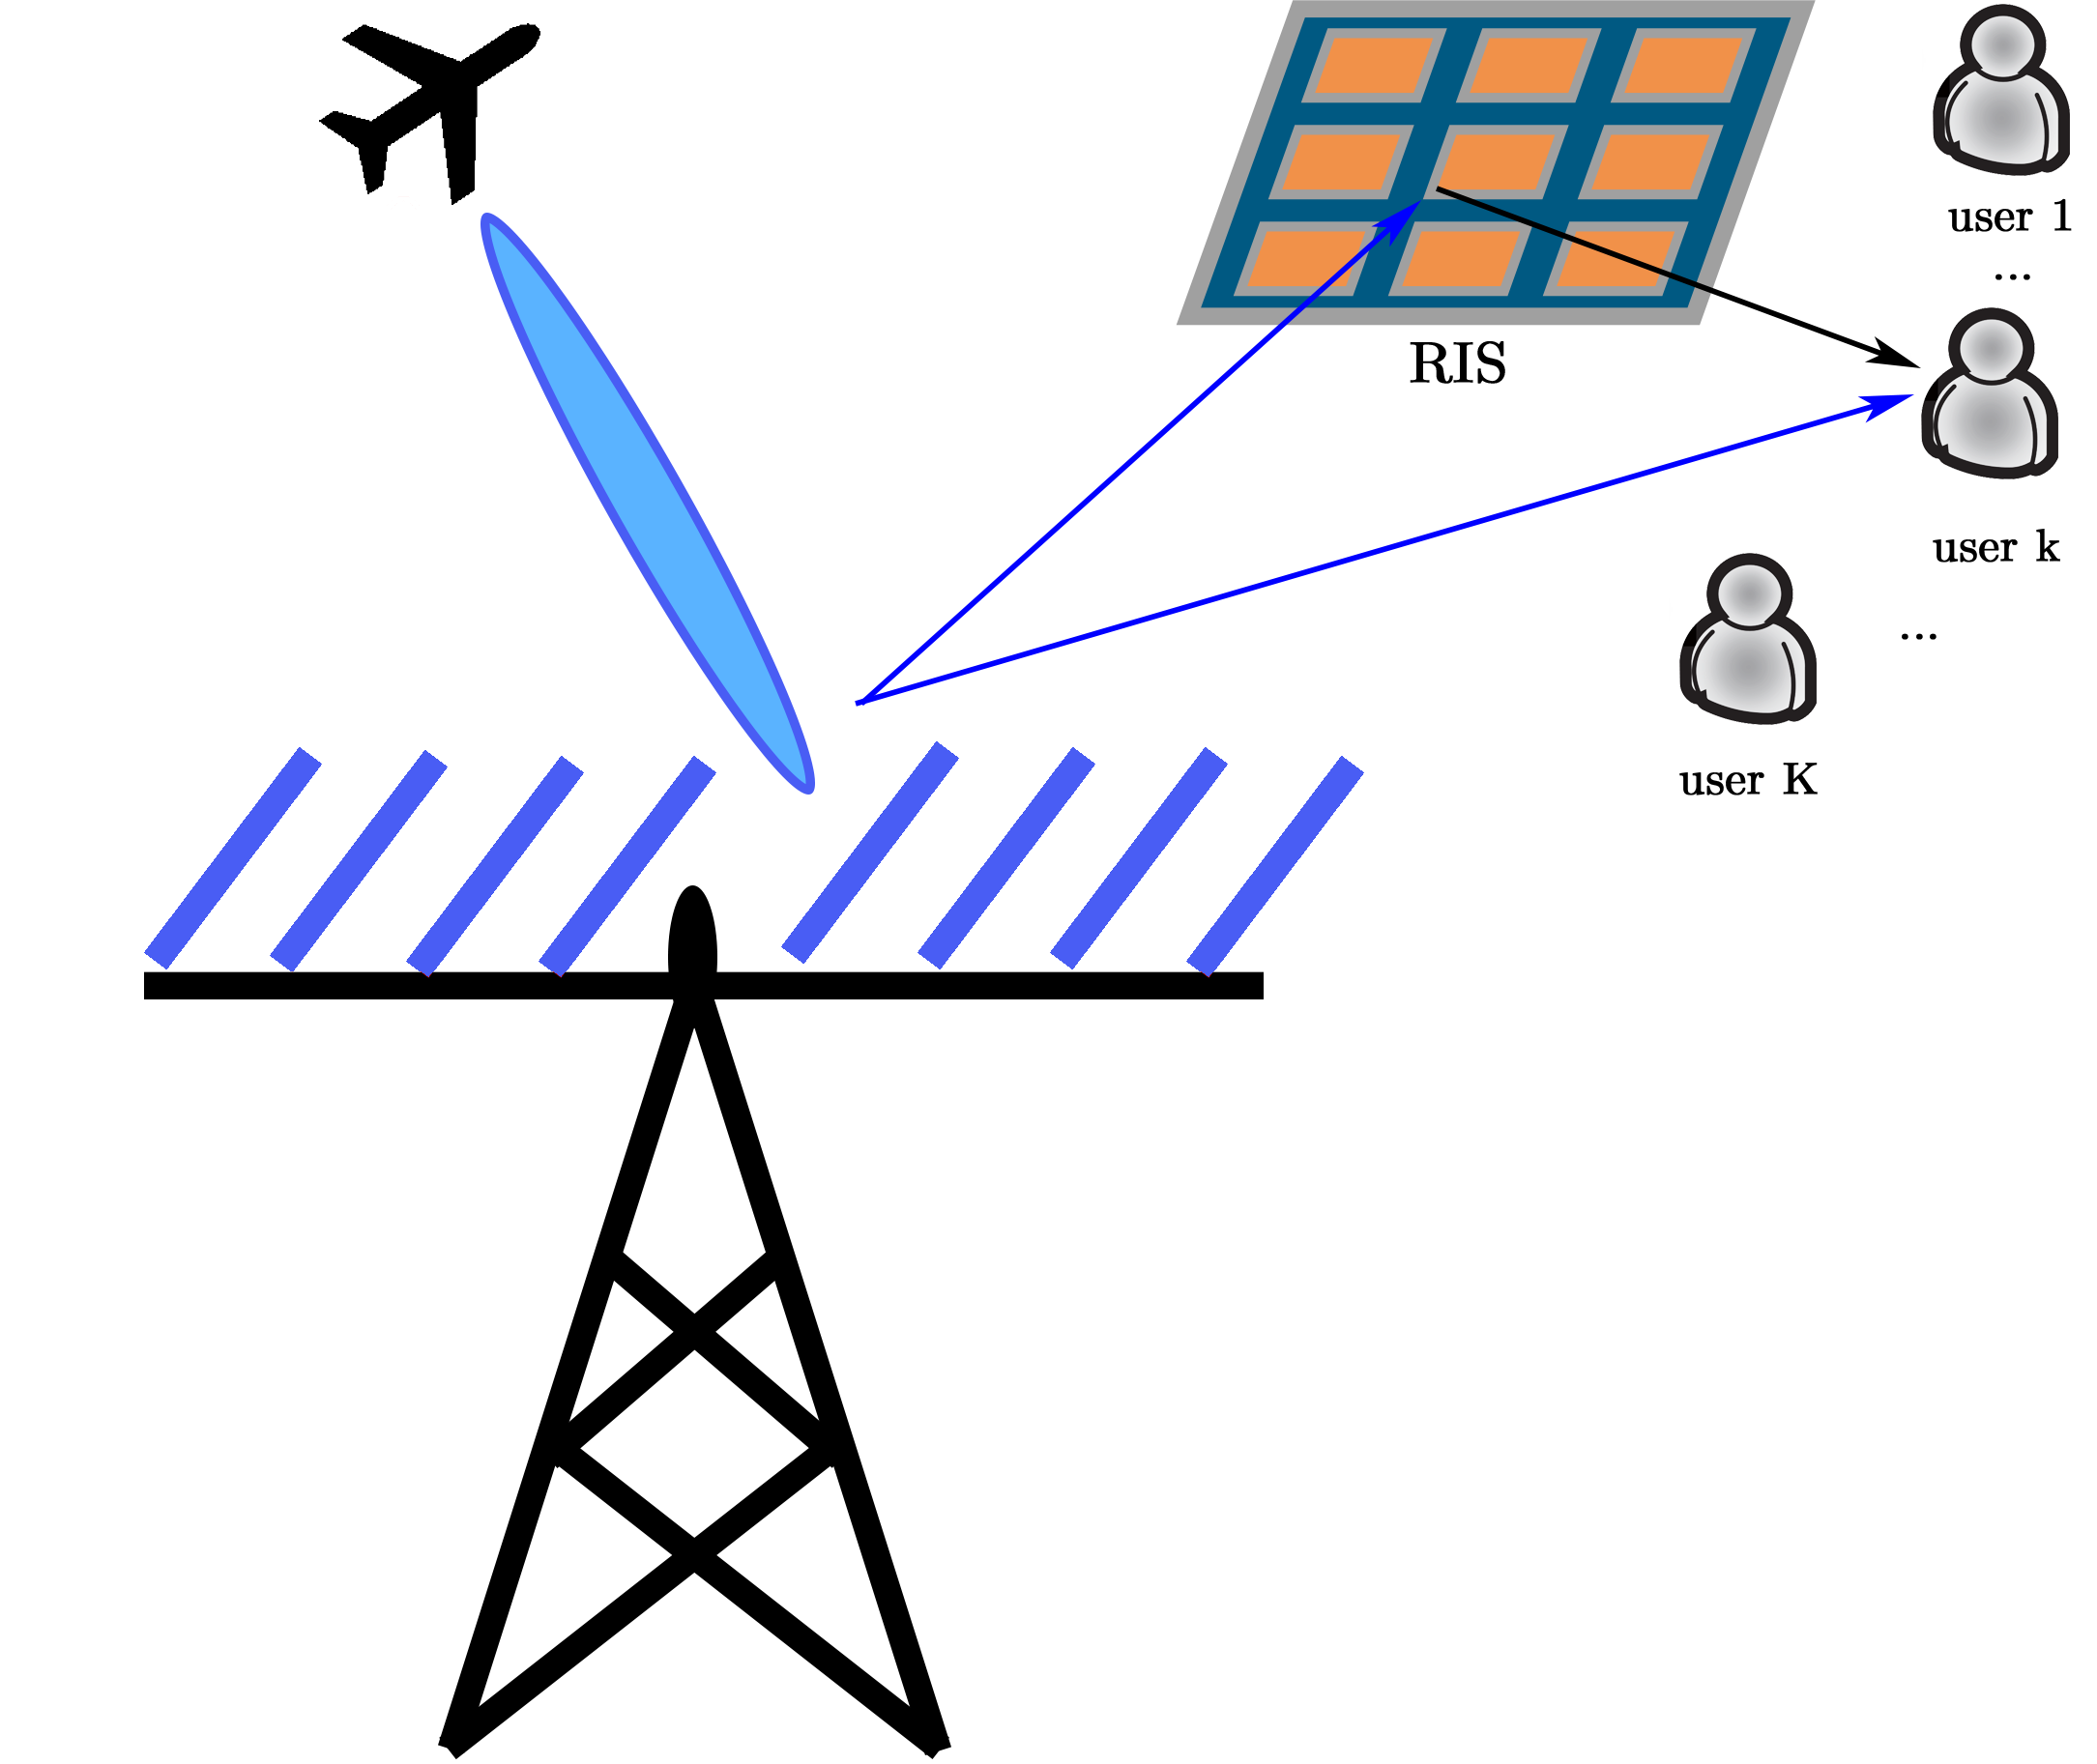
\includegraphics[width=0.42\textwidth]{./shared_setup.png}
%       \label{fig:setup_shared}
%   }
%   \caption{RIS-aided Dual-functional Radar and Communication system}
%   \label{fig:setup}
% \end{figure}

\section{System Model}\label{sec:system-model}
  As shown in Figure \ref{fig:setup}, we aim to investigate the RIS-aided MIMO radar
and MISO multi-user communications. This system serves $K$ users with a signal antenna, which receives
the signal from a BS equipped with $M$ antennas and a RIS equipped with $N$ reflecting elements.
The uniform linear antennas (ULA) are assumed to be the antenna deployment in this model.
The system also works in the tracking mode as a radar to tracking one target at the azimuth 
angle of $\varphi_m$. The overall power budget of this system is $P$. This system model partly follows the work \cite{xu2020tradeoff}.

\subsection{Separated Deployment}

In separated deployment, there are two groups of antennas: $M_r$ radar antennas and $M_c$ communication antennas, which transmit 
radar and communication signals separately. The power budgets of the radar and communications antennas are
$P_r$ and $P_c$, respectively.

The observation at user $k$ is given as
\begin{equation}
    x_k = (\mathbf{h}_k^H \mathbf{\Theta}^H \mathbf{H}_c + {\bf d}_{c,k}^H) \sum_{j=1}^K \mathbf{p}_j s_j + (\mathbf{h}_k^H \mathbf{\Theta}^H \mathbf{H}_r + {\bf d}_{r,k}^H) \mathbf{q} + n_k \label{eq1}
\end{equation}
where $\mathbf{h}_k \in \mathbb{C}^{N \times 1}$ is the channel from
RIS to user $k$, $\mathbf{H}_c \in \mathbb{C}^{N \times M_c}$ and $\mathbf{H}_r \in \mathbb{C}^{N \times M_r}$
are the channels from communication and radar antennas to RIS, respectively. The direct channels from communication 
and radar antennas to user $k$ are denoted by ${\bf d}_{c,k}$ and ${\bf d}_{r,k}$. $s_j$ is the 
information symbol for user $j$, and $n_k \sim \mathcal{CN}(0,\sigma_n^2)$ is the complex 
Gaussian noise at user $k$. The linear precoding
is exploited at the BS and $\mathbf{p}_j \in \mathbb{C}^{M_c \times 1}$ is the linear 
precoder for user $j$. $\mathbf{q} \in \mathbb{C}^{M_r \times 1}$ is the radar signals whose 
covariance matrix is ${\bf{R}}_{\bf q} = \mathbb{E}({\bf{q}}{\bf{q}}^H)$. 
$\mathbf{\Theta} \in \mathbb{C}^{N \times N}$ is the (reflecting) passive beamforming matrix at RIS,
which is modeled as group connected reconfigurable impedance network \cite{shen2020modeling}: 
\begin{align}
    {\bf \Theta} = \mathrm{diag}({\bf \Theta}_1,{\bf \Theta}_2,...,{\bf \Theta}_G) 
    \\ {\bf \Theta}_g = {\bf \Theta}_g^T, {\bf \Theta}_g^H{\bf \Theta}_g = {\bf I}, \forall g
\end{align}
where $G$ is the number of groups in the impedance network and ${\bf \Theta}_g \in \mathbb{C}^{N_G \times N_G}$ is a full matrix. 
$N_G = N / G$ is the number of elements in each group. If $G=1$, the RIS is a fully 
connected network; if $G=N$, the RIS is a single connected network.

The SINR and achievable rate at user $k$ are
\begin{align}
    &\gamma_k=\frac{|{\bf c}_k^H {\bf p}_k|^2}{\sum_{j=1,j \neq k}^K |{\bf c}_k^H {\bf p}_j|^2 + {\bf r}_k^H {\bf R}_{\bf q} {\bf r}_k + \sigma^2_n}\\
    &R_k = \log_2 ( 1 + \gamma_k )
\end{align}
where ${\bf c}_k = \mathbf{H}_c^H \mathbf{\Theta} \mathbf{h}_k+ {\bf d}_{c,k}$
and ${\bf r}_k= \mathbf{H}_r^H \mathbf{\Theta} \mathbf{h}_k + {\bf d}_{r,k}$.

We aim to maximize the WSR as well as the probing power in
direction $\varphi_m$. The WSR is given as
\begin{equation}
    R = \sum_{k=1}^K \mu_k R_k \label{eq5}
\end{equation}
where $\mu_k$ is the weight specified for user $k$ and is determined according the fairness and
quality of service (QoS) requirements.
The probing power in direction $\varphi_m$ is given as
\begin{equation}
    d(\varphi_m) = {\bf{a}}^H(\varphi_m) {\bf{C}} {\bf{a}}(\varphi_m) \label{eq6}
\end{equation}
where ${\bf a}(\varphi_m) \in \mathbb{C}^{M \times 1}$ is the steering 
vector. For ULA deployment, the steering vector is defined as
\begin{equation}
    {\bf{a}}(\varphi_m) = [1, e^{j\frac{2\pi}{\lambda}d\sin({\varphi_m})},...,e^{j\frac{2\pi}{\lambda}d(M-1)\sin({\varphi_m})}]^T \label{eq7}
\end{equation}
where $\lambda$ is the signal wavelength and $d$ is the antenna spacing. 
Without loss of generality, we set $d = \lambda / 2$. ${\bf{C}} \in \mathbb{C}^{M \times M}$ is the covariance matrix of 
the overall transmit signal. As the communication
and radar signals are uncorrelated, the covariance matrix is given as 
\begin{equation}
    {\bf{C}} = \left[\begin{matrix}
        {\bf{R}}_{\bf q} & \bf{0}\\
        \bf{0} & {\bf{P}}{\bf{P}}^H
    \end{matrix}\right] \label{eq8}
\end{equation}
where ${\bf P} = \begin{bmatrix} {\bf p}_1,...,{\bf p}_k\end{bmatrix} $

Therefore, \eqref{eq6} can be rewritten as
\begin{equation}
    d(\varphi_m) = {\bf{a}}_r^H(\varphi_m) {\bf{R}}_{\bf q} {\bf{a}}_r(\varphi_m) + {\bf{a}}_c^H(\varphi_m) {\bf{P}}{\bf{P}}^H {\bf{a}}_c(\varphi_m) \label{eq9}
\end{equation}
where ${\bf{a}}_r(\varphi_m)$ and ${\bf{a}}_c(\varphi_m)$ denote the steering vectors
of radar and communication antennas, respectively.

\subsection{Shared Deployment}

In shared deployment, all the $M$ antennas transmit communication signal. Therefore, the received signal at user $k$ is
\begin{equation}
    \check{x}_k = ({\bf h}_k^H {\bf \Theta}^H {\bf H} + {\bf d}_k^H) \sum_{j=1}^K \check{\bf p}_j s_j
\end{equation}
where ${\bf h}_k \in \mathbb{C}^{N \times 1}$, ${\bf H} \in \mathbb{C}^{M \times N}$, ${\bf d}_k \in \mathbb{C}^{M \time 1}$, 
${\bf \Theta} \in \mathbb{C}^{N \times N}$, $\check{\bf p}_j \in \mathbb{C}^{M \times 1}$, and $s_j \in \mathbb{C}$. 
The SINR at user $k$ is
\begin{equation}
    \check{\gamma}_k = \frac{|\check{\bf c}_k^H \check{\bf p}_k|^2}{\sum_{j=1,j\neq k}^K |\check{\bf c}_k^H \check{\bf p}_j|^2 + \sigma_n^2}
\end{equation}
where $\check{\bf c}_k = {\bf H}^H {\bf \Theta} {\bf h}_k + {\bf d}_k$. Thus, the WSR is
\begin{equation}
    \check{R} = \sum_{k=1}^K \mu_k \check{R}_k
\end{equation}
where $\check{R}_k = \log_2(1+\check{\gamma}_k)$ is the achievable rate at user $k$.

The probing power in direction of $\varphi_m$ is
\begin{equation}
    \check{d}(\varphi_m) = {\bf a}^H(\varphi_m) \sum_{j=1}^K {\bf p}_j {\bf p}_j^H {\bf a}(\varphi_m)
\end{equation}

\section{Problem Formulation}\label{sec:problem-formulation}
  In this project, the perfect channel state information (CSI) is assumed to be known. The CSI acquisition is
challenging in RIS-aided system because of the passive nature of RIS, which means it requires the estimation of 
a large number of unknown parameters cause by RIS \cite{liu2020RIS}. However, this problem can be tackled by deep learning 
techniques such as deep denoising neural network \cite{liu2020deep} or convolutional neural network \cite{elbir2020deep}.

When CSI is known, the problem of transmission optimization and RIS optimization in separated deployment is formulated as

\begin{subequations}\label{problem:seperated_problem}
    \begin{align}
        \label{eqn:seperated_problem_obj}
        \max_{\mathbf{P},\mathbf{R}_{\bf q},\mathbf{\Theta}} \quad  & \rho\sum_{k=1}^K \mu_k R_k(\mathbf{P},\mathbf{R}_{\bf q},\mathbf{\Theta}) + \mathbf{a}_r^H(\varphi_m)\mathbf{R}_{\bf q} \mathbf{a}_r(\varphi_m) 
         + \mathbf{a}_c^H(\varphi_m)\mathbf{P}\mathbf{P}^H\mathbf{a}_c(\varphi_m)\\
        \label{eqn:seperated_problem_constant_modulus} 
        \mathrm{s.t.} \quad &\mathrm{diag}(\mathbf{R}_{\bf q}) = \frac{P_r}{M_r}\mathbf{1}^{M_r \times 1},\\
        \label{eqn:seperated_problem_power_budget}
        &\mathrm{Tr} (\mathbf{P}\mathbf{P}^H) \leq P_c,\\
        \label{eqn:seperated_problem_semidefinite}
        &\mathbf{R}_{\bf q} \succeq 0, {\bf R}_{\bf q} = {\bf R}_{\bf q}^H, \\
        \label{eqn:seperated_problem_reflecting_1}
        &{\bf \Theta} = \mathrm{diag}({\bf \Theta}_1,{\bf \Theta}_2,...,{\bf \Theta}_G),\\
        \label{eqn:seperated_problem_reflecting_2}
        &{\bf \Theta}_g = {\bf \Theta}_g^T, {\bf \Theta}_g^H{\bf \Theta}_g = {\bf I}, \forall g,
    \end{align}
\end{subequations}
where the first part of \eqref{eqn:seperated_problem_obj} is the WSR and the rest is the probing power
in direction $\varphi_m$. Both of them are maximized with the regularization parameter $\rho$.
\eqref{eqn:seperated_problem_constant_modulus} is the constant-modulus constraint imposed by radar, so that the optimal
low peak-to-average power ratio is guaranteed and the radar signal distortion is therefore reduced \cite{liu2020tutorial}. 
\eqref{eqn:seperated_problem_power_budget} is the overall power budget constraint imposed by communications, and \eqref{eqn:seperated_problem_semidefinite}
constraints the covariance matrix ${\bf{R}}_{\bf q}$ to be Hermitian and positive semidefinite. The last two constraints
are imposed by the RIS. After finding the optimal ${\bf R_q}$, the radar signal can be obtained by the method in \cite{luo2010semidefinite}.

In shared deployment, the dual-function optimization problem is formulated as
\begin{subequations}\label{problem:shared_problem}
    \begin{align}
      \label{eqn:shared_problem_obj} 
      \max_{\check{\bf p}_1,...,\check{\bf p}_K} \quad &\rho \sum_{k=1}^K \mu_k \check{R}_k(\check{\bf p}_1,...,\check{\bf p}_K,{\bf \Theta}) 
      + {\bf a}^H(\varphi_m) \sum_{k=1}^K \check{\bf p}_k \check{\bf p}_k^H {\bf a}(\varphi_m)\\
      \label{eqn:shared_problem_constant_modulus} 
      \mathrm{s.t.} \quad &\mathrm{diag}\left( \sum_{k=1}^K \check{\bf p}_k \check{\bf p}_k^H \right) = \frac{P}{M}{\bf 1}^{M \times 1}, \\
      \label{eqn:shared_problem_reflecting_1} 
      & {\bf \Theta} = \mathrm{diag}({\bf \Theta}_1, {\bf \Theta}_2,..., {\bf \Theta}_G), \\
      \label{eqn:shared_problem_reflecting_2} 
      & {\bf \Theta}_{g}={\bf \Theta}_{g}^T, {\bf \Theta}_g^H {\bf \Theta}_g = {\bf I}, \forall g, 
    \end{align}
\end{subequations}
where the WSR and probing power are also maximized with regularization parameter $\rho$. \eqref{eqn:shared_problem_constant_modulus} 
is the constant-modulus constraint for MIMO radar. The overall power constraint is omitted because it is obviously satisfied when 
the constant modulus is met. The last two constraints are for generalized RIS.

The problems \eqref{problem:seperated_problem} and \eqref{problem:shared_problem} are essentially multi-objective optimization problems,
which can lead to the tradeoff between different objectives, i.e., WSR and probing power.


\section{WMMSE and Fractional Programming Based Algorithm}\label{sec:algorithms}
  It is clear that both \eqref{problem:seperated_problem} and \eqref{problem:shared_problem} are non-convex optimization problem.
However, we point out that they can be converted to
two optimization problems with respect to $\{{\bf{P}},{\bf{R}}_x\}$ and
$\bf{\Theta}$, respectively, using Weighted Minimum Mean Square Error (WMMSE) 
framework \cite{christensen2008weighted} and Fractional 
Programming (FP) \cite{shen2018fractional}. Then the optimal solution can be obtained in an alternative manner.

\subsection{Algorithm for Separated Deployment}

\subsubsection{WMMSE for Active Beamforming} \label{sec:WMMSE_separated}

Based on the WMMSE method proposed in \cite{christensen2008weighted}, the WSR 
maximization problem in \eqref{problem:seperated_problem} can be converted to an equivalent weight mean square
error (MSE) minimization problem via the following process.

The observation at user $k$ can be rewritten as
\begin{align} \label{eqn:separated_received_signal_transformed}
    x_k  & = {\bf c}_k^H \sum_{j=1}^K {\bf p}_j s_j +  {\bf r}_k^H {\bf q} + n_k \nonumber
    \\ & = {\bf c}_k^H {\bf p}_k s_k  + \underbrace{{\bf c}_k^H \sum_{j=1, j \neq k}^K {\bf p}_j s_j +  {\bf r}_k^H {\bf q}}_{\text{interference}} + n_k .
\end{align}
So the efficient noise plus interference power is 
\begin{equation} \label{eqn:separated_noise_interference}
    N_k=\sum_{j=1, j\neq k}^K |{\bf c}_k^H {\bf p}_j|^2 + {\bf r}_k^H {\bf R}_{\bf q} {\bf r}_k + \sigma^2_n.
\end{equation}
The estimated symbol using the receiver $g_k$ at user $k$ is
\begin{align} \label{eqn:separated_estimated}
    \hat{s}_k &= g_k x_k \nonumber\\
    &= g_k {\bf c}_k^H \sum_{j=1}^K {\bf p}_j s_j + g_k {\bf r}_k^H {\bf q} + g_k n_k.
\end{align}
The MSE is given as
\begin{align} \label{eqn:separated_mse}
    e_k  = & \mathbb{E} \Big[ \Vert \hat{s}_k - s_k \Vert^2 \Big] \nonumber\\
    = & |g_k|^2 \left( \sum_{j=1}^K | {\bf c}^H_k {\bf p}_j |^2 + {\bf r}_k^H {\bf R}_{\bf q} {\bf r}_k + \sigma_n^2 \right) - 2 \mathrm{Re}\left\{ g_k {\bf c}_k^H {\bf p}_k \right\} + 1.
\end{align}

The solution to the following unconstrained convex optimization problem yields the MMSE receiver.
\begin{align} \label{eqn:separated_mmse_receiver}
    g_k^{\mathrm{MMSE}} & = \arg \min_{g_k} e_k \nonumber
    \\ & = \frac{{\bf p}_k^H {\bf c}_k}{ | {\bf c}_k^H {\bf p}_k|^2 + N_k} \nonumber
    \\ & = \frac{{\bf p}_k^H {\bf c}_k}{\sum_{j=1, }^K |{\bf c}_k^H {\bf p}_j|^2 + {\bf r}_k^H {\bf R}_{\bf q} {\bf r}_k + \sigma^2_n}.
\end{align}
where $\partial e_k / \partial g_k = 0$ is the condition of the 
optimal MMSE receiver.

The MSE at the output of MMSE receiver is 
\begin{align} \label{eqn:separated_mmse_error}
    e_k^{\mathrm{MMSE}} & = \mathbb{E} \Big[(g_k^{\mathrm{MMSE}}x_k - s_k )(g_k^{\mathrm{MMSE}}x_k - s_k )^* \Big] \nonumber
    \\ & = \left(1+\frac{| {\bf c}_k^H {\bf p}_k|^2}{N_k} \right)^{-1} \nonumber
    \\ &= 1 - \frac{| {\bf c}_k^H {\bf p}_k|^2}{\sum_{j=1, }^K |{\bf c}_k^H {\bf p}_j|^2 + {\bf r}_k^H {\bf R}_{\bf q} {\bf r}_k + \sigma^2_n} .
\end{align} 

We can formulate another MSE minimization and probing power maximization problem, which is
\begin{subequations} \label{problem:separated_mse_minimization}
    \begin{align}
        \min_{\mathbf{P},\mathbf{R}_{\bf q}} \quad &  \rho \sum_{k=1}^K w_k e_k(\mathbf{P},\mathbf{R}_{\bf q}) -\mathbf{a}_r^H(\varphi_m)\mathbf{R}_{\bf q} \mathbf{a}_r(\varphi_m) - \mathbf{a}_c^H(\varphi_m)\mathbf{P}\mathbf{P}^H\mathbf{a}_c(\varphi_m)\\
        \mathrm{s.t.} \quad &\mathrm{diag}(\mathbf{R}_{\bf q}) = \frac{P_r \mathbf{1}^{M_r \times 1}}{M_r}, \\ 
        &\mathrm{Tr} (\mathbf{P}\mathbf{P}^H) \leq P_c, \\ 
        & \mathbf{R}_{\bf q} \succeq 0, {\bf R}_{\bf q} = {\bf R}_{\bf q}^H ,
    \end{align}
\end{subequations}
According to \cite{christensen2008weighted}, the problem \eqref{problem:separated_mse_minimization} has the 
same optimal solution of $\{{\bf{P}},{\bf{R}}_{\bf q}\}$ as \eqref{problem:seperated_problem} for fixed ${\bf \Theta}$ as long as
\begin{equation} \label{eqn:seperated_wmmse_weight}
    w_k = \mu_k (e_k^{\mathrm{MMSE}})^{-1}.
\end{equation}

Problem \eqref{problem:separated_mse_minimization} is still non-convex because of the last term. Based on the
transformation method in \cite{xu2020tradeoff}, the last term is equal to
\begin{align} \label{eqn:separated_transmission_power_transformed}
    &- \mathbf{a}_c^H(\varphi_m)\mathbf{P} \mathbf{P}^H \mathbf{a}_c(\varphi_m) =\sum_{k=1}^K \mathbf{p}_k^H \underbrace{\Big(M_c \mathbf{I} - \mathbf{a}_c(\varphi_m)\mathbf{a}_c^H(\varphi_m)\Big)}_{\mathbf{Z}(\varphi_m)}\mathbf{p}_k-M_c\times P_c.
\end{align}
It can be proved that ${\mathbf{Z}(\varphi_m)}$ is a positive semidefinite matrix,
therefore \eqref{eqn:separated_transmission_power_transformed} is a convex function. The problem \eqref{problem:separated_mse_minimization} can be reformulated as
\begin{subequations} \label{problem:separated_mse_minimization_transformed}
    \begin{align}
        \min_{\mathbf{P},\mathbf{R}_{\bf q}} \quad & \rho\sum_{k=1}^K w_k e_k(\mathbf{P},\mathbf{R}_{\bf q})- \mathbf{a}_r^H(\varphi_m)\mathbf{R}_{\bf q}\mathbf{a}_r(\varphi_m) +\sum_{k=1}^K\mathbf{p}_k^H \mathbf{Z}(\varphi_m)\mathbf{p}_k \\
        \mathrm{s.t.} \quad &\mathrm{diag}(\mathbf{R}_{\bf q}) = \frac{P_r \mathbf{1}^{M_r \times 1}}{M_r}, \\ 
        &\mathrm{Tr} (\mathbf{P}\mathbf{P}^H) \leq P_c ,\\ 
        & \mathbf{R}_{\bf q} \succeq 0, {\bf R}_{\bf q} = {\bf R}_{\bf q}^H .
    \end{align}
\end{subequations}

For the fixed $\bf{\Theta}$, the maximization of WSR and probing power can be solved by alternating 
between updating $w_k$ according to \eqref{eqn:seperated_wmmse_weight} and solving \eqref{problem:separated_mse_minimization_transformed}. 
The problem \eqref{problem:separated_mse_minimization_transformed} is an SDP that the CVX toolbox \cite{cvx} can effectively solve.


\subsubsection{Fractional Programming for Passive Beamforming} \label{sec:FP_separated}

For the fixed $\bf{P}$ and ${\bf{R}}_{\bf q}$, the problem \eqref{problem:seperated_problem} is simplified to
\begin{subequations} \label{problem:separated_theta}
    \begin{align}
        \max_{\mathbf{\Theta}} \quad & \sum_{k=1}^K \mu_k \log_2 ( 1 + \gamma_k (\mathbf{\Theta})) 
        \\ \mathrm{s.t.} \quad & {\bf \Theta} = \mathrm{diag}({\bf \Theta}_1,{\bf \Theta}_2,...,{\bf \Theta}_G) ,
        \\ &{\bf \Theta}_g = {\bf \Theta}_g^T, {\bf \Theta}_g^H{\bf \Theta}_g = {\bf I}, \forall g .
    \end{align}
\end{subequations}
The logarithmic fractional form of WSR and the quadratic equality constraint lead to the non-convexity of problem \eqref{problem:separated_theta}.
Nevertheless, we show that it can be tackled based on Lagrangian dual transform \cite{shen2018fractional2}, quadratic transform \cite{shen2018fractional},
and scattering-reactance relationship \cite{shen2020modeling}.

Applying the Lagrangian dual transform proposed in \cite{shen2018fractional2},
\eqref{problem:separated_theta} is equivalent to 
\begin{subequations} \label{problem:separated_theta_dual_transformed}
    \begin{align}
        \max_{\mathbf{\Theta},\boldsymbol{\alpha}} \quad & f(\mathbf{\Theta},\boldsymbol{\alpha}) = \sum_{k=1}^K\mu_k\log_2(1+\alpha_k)-\sum_{k=1}^K\mu_k\alpha_k +\sum_{k=1}^K \frac{\mu_k(1+\alpha_k)\gamma_k}{1+\gamma_k}\\
        \mathrm{s.t.} \quad &  {\bf \Theta} = \mathrm{diag}({\bf \Theta}_1,{\bf \Theta}_2,...,{\bf \Theta}_G) ,
        \\ &{\bf \Theta}_g = {\bf \Theta}_g^T, {\bf \Theta}_g^H{\bf \Theta}_g = {\bf I}, \forall g.
    \end{align}
\end{subequations}

% \begin{align}
%     f(\mathbf{\Theta},\boldsymbol{\alpha})=&\sum_{k=1}^K\mu_k\log_2(1+\alpha_k)-\sum_{k=1}^K\mu_k\alpha_k +\sum_{k=1}^K \frac{\mu_k(1+\alpha_k)\gamma_k}{1+\gamma_k} \label{eq21}
% \end{align}

For fixed $\bf{\Theta}$, \eqref{problem:separated_theta_dual_transformed} is an unconstrained convex optimization
problem with respect to $\boldsymbol{\alpha} = [\alpha_1,...,\alpha_K]$ and the optimal $\boldsymbol{\alpha}^\star$ is given as
\begin{equation} \label{eqn:separated_optimal_alpha}
    \alpha^\star_k=\gamma_k,
\end{equation}
which is obtained from ${\partial f}/{\partial \alpha_k} = 0$.

For the fixed $\boldsymbol{\alpha}$, \eqref{problem:separated_theta_dual_transformed} can be simplified to a fractional form
\begin{subequations} \label{problem:separated_theta_fractional_form}
    \begin{align}
        \max_{\mathbf{\Theta}} \quad & \sum_{k=1}^K \frac{\mu_k(1+\alpha_k)\gamma_k}{1+\gamma_k}\\
        \mathrm{s.t.} \quad & {\bf \Theta} = \mathrm{diag}({\bf \Theta}_1,{\bf \Theta}_2,...,{\bf \Theta}_G) ,
        \\ &{\bf \Theta}_g = {\bf \Theta}_g^T, {\bf \Theta}_g^H{\bf \Theta}_g = {\bf I}, \forall g,
    \end{align}
\end{subequations}
where the logarithm in \eqref{problem:separated_theta} is removed. The problem \eqref{problem:separated_theta_fractional_form} 
is a sum-of-ratios FP problem. To apply the quadratic transform
proposed in \cite{shen2018fractional}, we firstly reformulated the objective function
of \eqref{problem:separated_theta_fractional_form} by letting $\boldsymbol{\theta} = \mathrm{vec}({\bf \Theta}^T)$:

\begin{align}
    g(\boldsymbol{\theta})
    =&\sum_{k=1}^K \frac{\mu_k(1+\alpha_k)\gamma_k}{1+\gamma_k} \nonumber\\ 
    =&\sum_{k=1}^K\frac{\mu_k(1+\alpha_k)|{\bf c}_{k}^H \mathbf{p}_k|^2} {\sum_{j=1}^{K} |{\bf c}_k^H \mathbf{p}_j|^2 + {\bf r}_k^H \mathbf{R}_{\bf q} {\bf r}_k + \sigma^2_n} \nonumber \\ 
    =&\sum_{k=1}^K\frac{\mu_k(1+\alpha_k)|({\boldsymbol \theta}^H {\bf A}_k \mathbf{H}_c + {\bf d}_{c,k}^H) \mathbf{p}_k|^2} {\sum_{j=1}^{K} |({\boldsymbol \theta}^H {\bf A}_k\mathbf{H}_c + {\bf d}_{c,k}^H) \mathbf{p}_j|^2 + ({\boldsymbol \theta}^H {\bf A}_k \mathbf{H}_r + {\bf d}_{r,k}^H) \mathbf{R}_{\bf q} (\mathbf{H}_r^H {\bf A}_k^H {\boldsymbol \theta}+ {\bf d}_{r,k}) + \sigma_n^2} .
\end{align}
The matrix ${\bf A}_k$ is defined as
\begin{equation}
    {\bf A}_k = \left[{\bf J}^0 \tilde{\bf h}_k,  {\bf J}^N \tilde{\bf h}_k,{\bf J}^{2 N} \tilde{\bf h}_k,...,{\bf J}^{(N-1) N} \tilde{\bf h}_k \right],
\end{equation}
where 
\begin{align}
    &\tilde{\bf h}_k = [ {\bf h}_k^H, {\bf 0}_{(N-1)N}^T]^T \in \mathbb{C}^{NN\times 1}, 
    \\ &{\bf J} = \left[ \begin{matrix} {\bf 0}_{NN-1}^T & 0 \\ {\bf I}_{NN-1} & {\bf 0}_{NN-1}\end{matrix} \right].
\end{align}
The $g(\boldsymbol{\theta})$ can be further simplified to
\begin{align}
    g(\boldsymbol{\theta}) = \sum_{k=1}^K \frac{\mu_k(1+\alpha_k) |\boldsymbol{\theta}^H {\bf a}_{k,k} + b_{k,k}|^2}{\sum_{j=1}^K |\boldsymbol{\theta}^H {\bf a}_{j,k} + b_{j,k}|^2 + \boldsymbol{\theta}^H {\bf B}_k \boldsymbol{\theta} +  2 \mathrm{Re} \left\{ \boldsymbol{\theta}^H {\bf f}_k \right\} + m_k},
\end{align}
where
\begin{align} 
    &\mathbf{a}_{j,k}={\bf A}_k \mathbf{H}_c \mathbf{p}_j, 
    \\ &b_{j,k} = {\bf d}_{c,k}^H {\bf p}_j, 
    \\ &\mathbf{B}_k={\bf A}_k\mathbf{H}_r \mathbf{R}_{\bf q} \mathbf{H}_r^H {\bf A}_k^H, 
    \\ &{\bf f}_k = {\bf A}_k {\bf H}_r {\bf R}_{\bf q} {\bf d}_{r,k}, 
    \\ &m_k = {\bf d}_{r,k}^H {\bf R}_{\bf q} {\bf d}_{r.k} + \sigma^2_n.
\end{align}
As $\mathbf{R}_{\bf q}$ is positive semidefinite, it can be written as $\mathbf{R}_{\bf q}=\mathbf{R}_d^H \mathbf{R}_d$.
Therefore, we have $\mathbf{B}_k=(\mathrm{diag}\{\mathbf{h}_k^H\} \mathbf{H}_r \mathbf{R}_d^H)(\mathrm{diag}\{\mathbf{h}_k^H\} \mathbf{H}_r \mathbf{R}_d^H)^H$,
which indicates that $\mathbf{B}_k$ is positive semidefinite.

Applying the quadratic transform of FP proposed in \cite{shen2018fractional}, 
the objective function $g(\boldsymbol{\theta})$ in \eqref{problem:separated_theta_fractional_form} 
is transformed to a new function $h(\boldsymbol{\theta}, {\bf y})$ with ${\bf y} = [y_1,...,y_K]^T$.

\begin{align}
    h(\boldsymbol{\theta}, {\bf y}) = & \sum_{k=1}^K\left( 2 \mathrm{Re} \left\{ y_k^* \sqrt{\mu_k (1+\alpha_k)} \left( \boldsymbol{\theta}^H {\bf a}_{k,k} + b_{k,k} \right) \right\} \right)  \nonumber\\
    & -\sum_{k=1}^K |y_k|^2 \left(\sum_{j=1}^K |\boldsymbol{\theta}^H {\bf a}_{j,k} + b_{j,k}|^2 + \boldsymbol{\theta}^H {\bf B}_k \boldsymbol{\theta} + 2 \mathrm{Re} \left\{ \boldsymbol{\theta}^H {\bf f}_k \right\} + m_k \right). 
\end{align}

The problem \eqref{problem:separated_theta_fractional_form} is equivalent to 
\begin{subequations}\label{problem:separated_theta_quadratic_transform}
    \begin{align} 
        \max_{\boldsymbol{\theta},\mathbf{y}} \quad & h(\boldsymbol{\theta}, {\bf y}) \\  
        \mathrm{s.t.} \quad &  \boldsymbol{\theta} = \mathrm{vec}({\bf \Theta}^T),
        \\ & {\bf \Theta} = \mathrm{diag}({\bf \Theta}_1,{\bf \Theta}_2,...,{\bf \Theta}_G) ,
        \\ &{\bf \Theta}_g = {\bf \Theta}_g^T, {\bf \Theta}_g^H{\bf \Theta}_g = {\bf I}, \forall g,
        \\ & {\bf y} = [y_1,...,y_K]^T, y_k \in \mathbb{C}, \forall k.
    \end{align}
\end{subequations}

For fixed $\boldsymbol{\theta}$, \eqref{problem:separated_theta_quadratic_transform} is an unconstrained convex problem
with respect to $\bf{y}$. By setting $\partial h / \partial y_k$ to zero, we can get the optimal solution:
\begin{equation} \label{eqn:separated_optimal_y}
    y^\star_k = \frac{\sqrt{\mu_k (1+\alpha_k)} \left(\boldsymbol{\theta}^H {\bf a}_{k,k} + b_{k,k} \right)}{\sum_{j=1}^K |\boldsymbol{\theta}^H {\bf a}_{j,k} + b_{j,k}|^2 + \boldsymbol{\theta}^H {\bf B}_k \boldsymbol{\theta} + 2 \mathrm{Re} \left\{ \boldsymbol{\theta}^H {\bf f}_k \right\} + m_k}.
\end{equation}

For fixed $\bf{y}$, the term $|\boldsymbol{\theta}^H {\bf a}_{j,k} + b_{j,k}|^2$ in $h(\boldsymbol{\theta}, {\bf y})$
 can be rephrased as
\begin{align}
    &|\boldsymbol{\theta}^H {\bf a}_{j,k} + b_{j,k}|^2 \nonumber\\
    = &(\boldsymbol{\theta}^H {\bf a}_{j,k} + b_{j,k}) ( {\bf a}_{j,k}^H\boldsymbol{\theta} + b_{j,k}^*) \nonumber \\
    = &\boldsymbol{\theta}^H {\bf a}_{j,k} {\bf a}_{j,k}^H \boldsymbol{\theta} + 2 \mathrm{Re} \left\{ b_{j,k}^* \boldsymbol{\theta}^H {\bf a}_{j,k}  \right\} + |b_{j,k}|^2 .
\end{align}
Substituting this into $h(\boldsymbol{\theta}, {\bf y})$ and dropping the constant term, we get a new objective function
\begin{equation}
    \tilde{h}(\boldsymbol{\theta}) = -\boldsymbol{\theta}^H {\bf U} \boldsymbol{\theta} + 2 \mathrm{Re} \left\{ \boldsymbol{\theta}^H {\bf v} \right\},
\end{equation}
where 
\begin{align}
    &{\bf U} = \sum_{k=1}^K |y_k|^2 \left({\bf B}_k + \sum_{j=1}^K {\bf a}_{j,k} {\bf a}_{j,k}^H  \right), \\
    &{\bf v} = \sum_{k=1}^K \left( y_k^* \sqrt{\mu_k(1+\alpha_k)} {\bf a}_{k,k} - |y_k|^2 \left( {\bf f}_k + \sum_{j=1}^K b_{j,k}^* {\bf a}_{j,k} \right) \right).
\end{align}

Thus, the problem \eqref{problem:separated_theta_quadratic_transform} for fixed ${\bf y}$ is simplified to
\begin{subequations} \label{problem:separated_theta_quadratic_form}
    \begin{align}
        \min_{\boldsymbol{\theta}} \quad & \boldsymbol{\theta}^H {\bf U} \boldsymbol{\theta} - 2 \mathrm{Re} \left\{ \boldsymbol{\theta}^H {\bf v} \right\}\\  
        \mathrm{s.t.} \quad &  \boldsymbol{\theta} = \mathrm{vec}({\bf \Theta}^T)
        \\ &{\bf \Theta} = \mathrm{diag}({\bf \Theta}_1,{\bf \Theta}_2,...,{\bf \Theta}_G), 
        \\ &{\bf \Theta}_g = {\bf \Theta}_g^T, {\bf \Theta}_g^H{\bf \Theta}_g = {\bf I}, \forall g.
    \end{align}
\end{subequations}

As ${\bf{B}}_k$ is positive semidefinite, ${\bf U}$ is also positive semidefinite. Therefore, the objective functions of
\eqref{problem:separated_theta_quadratic_form} is convex. However, constrains are still non-convex. In order to tackle this problem, we follow the 
method proposed in \cite{shen2020modeling}, where the relationship between ${\bf \Theta}_g$ and 
reactance matrix ${\bf Z}_{I,g}$ is exploited, that is
\begin{align}
    &{\bf \Theta}_g = (j{\bf Z}_{I,g} + R_0 {\bf I})^{-1}(j{\bf Z}_{I,g} - R_0 {\bf I}), \forall g, 
    \\ &{\bf Z}_{I,g} = {\bf Z}_{I,g}^T, \forall g,
\end{align}
where $R_0$ refers to the characteristic impedance and is usually set as $R_0=50 \Omega$. The problem \eqref{problem:separated_theta_quadratic_form} can be 
rewritten as
\begin{subequations} \label{problem:separated_theta_unconstraint}
    \begin{align}
        \min_{\boldsymbol{\theta}} \quad & \boldsymbol{\theta}^H {\bf U} \boldsymbol{\theta} - 2 \mathrm{Re} \left\{ \boldsymbol{\theta}^H {\bf v} \right\}\\  
        \mathrm{s.t.} \quad &  \boldsymbol{\theta} = \mathrm{vec}({\bf \Theta}^T)
        \\ &{\bf \Theta} = \mathrm{diag}({\bf \Theta}_1,{\bf \Theta}_2,...,{\bf \Theta}_G),
        \\ &{\bf \Theta}_g = (j{\bf Z}_{I,g} + R_0 {\bf I})^{-1}(j{\bf Z}_{I,g} - R_0 {\bf I}), \forall g, 
        \\ &{\bf Z}_{I,g}={\bf Z}_{I,g}^T, \forall g.
    \end{align}
\end{subequations}
The objective of \eqref{problem:separated_theta_unconstraint} is essentially a function of ${\bf Z}_{I,g}$. Because ${\bf Z}_{I,g}$ can be arbitrary real symmetric
matrix, \eqref{problem:separated_theta_unconstraint} is an unconstrained optimization problem that can be addressed by utilising the Quasi-Newton method 
to optimize the upper triangular part of ${\bf Z}_{I,g}$.

In the special case where $G = N$, i.e., single connected network, the passive beamforming matrix ${\bf \Theta}$ is a diagonal matrix
given as 
\begin{equation}
    {\bf \Theta} = \mathrm{diag} \{ \theta_1,...,\theta_N \},
\end{equation}
where $|\theta_i| \leq 1, i=1,...N$. Following the same path of deriving \eqref{problem:separated_theta_unconstraint}, the following Quadratic Programme (QP)
can be obtained.
\begin{subequations} \label{problem:separated_theta_single}
    \begin{align}
        \min_{\boldsymbol{\breve \theta}} \quad & \boldsymbol{\breve \theta}^H \breve{\bf U} \boldsymbol{\breve \theta} - 2 \mathrm{Re} \left\{ \boldsymbol{\breve \theta}^H \breve{\bf v} \right\}\\  
        \mathrm{s.t.} \quad &  \boldsymbol{\breve \theta} = [\theta_1,...,\theta_N]^T,
        \\ &|\theta_i| \leq 1, \forall i,
    \end{align}
\end{subequations}
where 
\begin{align}
    &\breve{\bf U} = \sum_{k=1}^K |\breve{y}_k|^2 \left(\breve{\bf B}_k + \sum_{j=1}^K \breve{\bf a}_{j,k} \breve{\bf a}_{j,k}^H  \right), \\
    &\breve{\bf v} = \sum_{k=1}^K \left( \breve{y}_k^* \sqrt{\mu_k(1+\alpha_k)} \breve{\bf a}_{k,k} - |\breve{y}_k|^2 \left( \breve{\bf f}_k + \sum_{j=1}^K b_{j,k}^* \breve{\bf a}_{j,k} \right) \right), \\
    \label{eqn:separated_optimal_y_single}
    &\breve{y}_k = \frac{\sqrt{\mu_k (1+\alpha_k)} \left(\boldsymbol{\theta}^H \breve{\bf a}_{k,k} + b_{k,k} \right)}{\sum_{j=1}^K |\boldsymbol{\theta}^H \breve{\bf a}_{j,k} + b_{j,k}|^2 + \boldsymbol{\theta}^H \breve{\bf B}_k \boldsymbol{\theta} + 2 \mathrm{Re} \left\{ \boldsymbol{\theta}^H \breve{\bf f}_k \right\} + m_k},\\
    &\breve{\bf{a}}_{j,k}=\mathrm{diag}\{\mathbf{h}_k^H\} \mathbf{H}_c \mathbf{p}_j, \\
    &\breve{\bf{B}}_k=\mathrm{diag}\{\mathbf{h}_k^H\}\mathbf{H}_r \mathbf{R}_{\bf q} \mathbf{H}_r^H\mathrm{diag}\{\mathbf{h}_k\}, \\
    &\breve{\bf f}_k = \mathrm{diag} \{{\bf h}_k^H\} {\bf H}_r {\bf R}_{\bf q} {\bf d}_{r,k}.\\
\end{align}
The matrix $\breve{\bf U}$ can also be proved to be positive semidefinite, therefore \eqref{problem:separated_theta_single} is a convex QP.
Similar to SDP, QP can also be solved by CVX toolbox \cite{cvx}. 

Therefore, we propose a WMMSE-FP-based AO algorithm to solve the problem \eqref{problem:seperated_problem}.
The details are shown in Algorithm \ref{alg:A}


\begin{algorithm}[htb]
    \caption{WMMSE-FP-based AO Algorithm for Separated Deployment}
    \label{alg:A}
    \begin{algorithmic}[1]
        \REQUIRE{$t = 0$, ${\bf{P}}^{[t]}$, ${\bf{R}}_{\bf q}^{[t]}$, ${\bf{\Theta}}^{[t]}$;}
        \STATE{Calculate $\text{WSR}^{[t]}$ from ${\bf{P}}^{[t]}$, ${\bf{R}}_{\bf q}^{[t]}$ and ${\bf{\Theta}}^{[t]}$;} 
        \REPEAT 
        \STATE{$t = t+1$}
        \STATE{Calculate $g_k^{[t]}$ by \eqref{eqn:separated_mmse_receiver};}
        \STATE{Calculate $w_k^{[t]}$ by \eqref{eqn:seperated_wmmse_weight};}
        \STATE{Update active beamforming ${\bf{P}}^{[t]}$ and radar covariance matrix ${\bf{R}}_{\bf q}^{[t]}$ by solving \eqref{problem:separated_mse_minimization_transformed};}

        \STATE{Calculate $\alpha_k^{[t]}$ by \eqref{eqn:separated_optimal_alpha};}
        \STATE{Calculate $y_k^{[t]}$ by \eqref{eqn:separated_optimal_y} for group/fully connected RIS or $\breve{y}_k^{[t]}$ by \eqref{eqn:separated_optimal_y_single} for single connected RIS;}
        \STATE{Update ${\bf{\Theta}}^{[t]}$ by solving \eqref{problem:separated_theta_unconstraint} for group/fully connected RIS or \eqref{problem:separated_theta_single} for single connected RIS;}

        \STATE{Calculate $\text{WSR}^{[t]}$ from ${\bf{P}}^{[t]}$, ${\bf{R}}_{\bf q}^{[t]}$ and ${\bf{\Theta}}^{[t]}$;}

        \UNTIL{$\left|\text{WSR}^{[t-1]} - \text{WSR}^{[t]}\right| \leq \epsilon$.}

    \end{algorithmic}
\end{algorithm}

\subsection{Algorithm for Shared Deployment}

For fixed ${\bf \Theta}$, we firstly follow the same path in Section \ref{sec:WMMSE_separated} and reformulate \eqref{problem:shared_problem} using WMMSE as
\begin{subequations} \label{problem:shared_mse_minimization}
    \begin{align} 
        \min_{\check{\bf p}_1,...,\check{\bf p}_K} \quad &\rho \sum_{k=1}^K \check{w}_k \check{e}_k(\check{\bf p}_1,...,\check{\bf p}_K) +  \sum_{k=1}^K \check{\bf p}_k^H {\bf Z}(\varphi_m) \check{\bf p}_k  
        \\ \mathrm{s.t.} \quad &\mathrm{diag}\left( \sum_{j=1}^K \check{\bf p}_j \check{\bf p}_j^H \right) = \frac{P}{M} {\bf 1}^{M \times 1}, 
    \end{align}
\end{subequations}
where
\begin{align} 
    &\check{e}_k = |\check{g}_k|^2 \left( \sum_{j=1}^K |\check{\bf c}_k^H \check{\bf p}_j|^2 + \sigma_n^2 \right) - 2\mathrm{Re}\{ g_k \check{\bf c}_k^H \check{\bf p}_k\} + 1, \\
    \label{eqn:shared_mmse_receiver}
    &\check{g}_k^{\mathrm {MMSE}} = \frac{\check{\bf p}_k^H \check{\bf c}_k}{\sum_{j=1}^K |\check{\bf c}_k^H \check{\bf p}_j|^2 + \sigma_n^2},\\
    &\check{e}_k^{\mathrm{MMSE}} = 1-\frac{|\check{\bf c}_k^H \check{\bf p}_k|^2}{\sum_{j=1}^K |\check{\bf c}_k^H \check{\bf p}_j|^2 + \sigma_n^2},\\
    \label{eqn:shared_wmmse_weight}
    &\check{w}_k = \mu_k (\check{e}^{\mathrm{MMSE}})^{-1}, \\
    & {\bf Z}(\varphi_m) = \Big( M{\bf I} - {\bf a}(\varphi_m){\bf a}^H(\varphi_m) \Big).
\end{align}
The non-convexity of this problem is from the quadratic equality constraint. In \cite{xu2020tradeoff}, the authors proposed an MM algorithm to address it.
But the MM is an iterative algorithm, which leads to high complexity when it is nested in an outer iterative loop.
Thus, we propose a new low complexity algorithm based on SDR, which is capable of solving this problem in one step.   
Observing that this problem is an inhomogeneous QCQP, we firstly homogenize this problem.

The $\check{e}_k$ can be rewritten as
\begin{align}
    \check{e}_k &= |\check{g}_k|^2 \left( \sum_{j=1}^K |\check{\bf c}_k^H \check{\bf p}_j|^2 + \sigma_n^2 \right) - 2\mathrm{Re}\{ \check{g}_k \check{\bf c}_k^H \check{\bf p}_k\} + 1 \nonumber
    \\ & = |\check{g}_k|^2 \sum_{j=1}^K \check{\bf p}_j^H \check{\bf c}_k \check{\bf c}_k^H \check{\bf p}_j + |\check{g}_k|^2\sigma_n^2 - \check{g}_k \check{\bf c}_k^H \check{\bf p}_k - \check{g}_k^*\check{\bf p}_k^H \check{\bf c}_k + 1
\end{align}
Omit the constants and reformulate it as
\begin{align} 
    \hat{e}_k & = |\check{g}_k|^2 \sum_{j=1}^K \check{\bf p}_j^H \check{\bf c}_k \check{\bf c}_k^H \check{\bf p}_j  - \check{g}_k \check{\bf c}_k^H \check{\bf p}_k - \check{g}_k^* \check{\bf p}_k^H \check{\bf c}_k \nonumber
    \\ &=|\check{g}_k|^2\sum_{j=1,j\neq k}^K \check{\bf p}_j^H \check{\bf c}_k \check{\bf c}_k^H \check{\bf p}_j +|\check{g}_k|^2 \check{\bf p}_k^H \check{\bf c}_k \check{\bf c}_k^H \check{\bf p}_k - \check{g}_k \check{\bf c}_k^H \check{\bf p}_k - \check{g}_k^* \check{\bf p}_k^H \check{\bf c}_k \nonumber
    \\ & = \sum_{j=1,j \neq k}^K \begin{bmatrix} \hat{\bf p}_j^H & t_j^*\end{bmatrix} \begin{bmatrix} |\check{g}_k|^2 \check{\bf c}_k \check{\bf c}_k^H & {\bf 0} \\ {\bf 0}^T & 0 \end{bmatrix}  \begin{bmatrix} \hat{\bf p}_j \\ t_j\end{bmatrix} + \begin{bmatrix}   \hat{\bf p}_k^H & t_k^*\end{bmatrix}\begin{bmatrix} |\check{g}_k|^2 \check{\bf c}_k \check{\bf c}_k^H & -\check{g}_k^*\check{\bf c}_k \\ -\check{g}_k \check{\bf c}_k^H & 0 \end{bmatrix} \begin{bmatrix} \hat{\bf p}_k \\ t_k \end{bmatrix} 
\end{align}
where $|t_j|^2 = 1$ and $\hat{\bf p}_j = t_j \check{\bf p}_j$.

Similarly, we have
\begin{equation}
    \check{\bf p}_k^H {\bf Z}(\varphi_m) \check{\bf p}_k = \begin{bmatrix} \hat{\bf p}_k^H & t_k^* \end{bmatrix} \begin{bmatrix} {\bf Z}(\varphi_m) & {\bf 0} \\ {\bf 0}^T & 0 \end{bmatrix} \begin{bmatrix} \hat{\bf p}_k \\ t_k \end{bmatrix}
\end{equation}

The constraint can also be rewritten as
\begin{align}
    \mathrm{diag}&\left( \sum_{j=1}^K \check{\bf p}_j \check{\bf p}_j^H \right) = \frac{P}{M}{\bf 1}^{M \times 1} \nonumber\\
    &\Longrightarrow\mathrm{diag} \left( \sum_{j=1}^K \begin{bmatrix} \hat{\bf p}_j \\ t_j\end{bmatrix} \begin{bmatrix} \hat{\bf p}_j^H & t_j^* \end{bmatrix}\right)  = \begin{bmatrix} \frac{P}{M} {\bf 1}^{M \times 1} \\ \sum_{j=1}^K |t_j|^2\end{bmatrix} = \begin{bmatrix} \frac{P}{M} {\bf 1}^{M \times 1} \\ K\end{bmatrix}
\end{align}

Therefore, we can obtain a new homogenous QCQP optimization problem
\begin{subequations} \label{problem:shared_homogeneous_qcqp}
    \begin{align} 
        \min_{\tilde{\bf p}_1,...\tilde{\bf p}_K} \quad & \sum_{k=1}^K \left(\hat{w}_k\sum_{j=1,j \neq k}^K \tilde{\bf p}_j^H {\bf C}_{k,1}\tilde{\bf p}_j + \hat{w}_k\tilde{\bf p}_k^H {\bf C}_{k,2} \tilde{\bf p}_k + \tilde{\bf p}_k^H \hat{\bf Z}(\varphi_m) \tilde{\bf p}_k \right) 
        \\ \mathrm{s.t.} \quad & \mathrm{diag} \left( \sum_{k=1}^K \tilde{\bf p}_k \tilde{\bf p}_k^H \right) = \begin{bmatrix} \frac{P}{M} {\bf 1}^{M \times 1} \\ K\end{bmatrix}, 
        \\ &|[\tilde{\bf p}_k]_{M+1}|^2 =1, k=1,...,K, 
    \end{align}
\end{subequations}
where 
\begin{align} 
    & \hat{w}_k = \rho \check{w}_k,
    \\ & \tilde{\bf p}_k = \begin{bmatrix} \hat{\bf p}_k \\ t_k\end{bmatrix},
    \\ & {\bf C}_{k,1} = \begin{bmatrix} |\check{g}_k|^2 \check{\bf c}_k \check{\bf c}_k^H & {\bf 0} \\ {\bf 0}^T & 0 \end{bmatrix},
    \\ & {\bf C}_{k,2} = \begin{bmatrix} |\check{g}_k|^2 \check{\bf c}_k \check{\bf c}_k^H & -\check{g}_k^* \check{\bf c}_k \\ -\check{g}_k \check{\bf c}_k^H & 0 \end{bmatrix}, 
    \\ &\hat{\bf Z}(\varphi_m) = \begin{bmatrix} {\bf Z}(\varphi_m) & {\bf 0} \\ {\bf 0}^T & 0 \end{bmatrix},
\end{align}
and $[\tilde{\bf p}_k]_{M+1}$ denotes the $(M+1)$-th element of $\tilde{\bf p}_k$.

Letting ${\bf T}_k = \tilde{\bf p}_k \tilde{\bf p}_k^H$ and omitting the rank-one constraint, we obtain the SDR of the 
homogenous QCQP problem:
\begin{subequations} \label{problem:shared_sdr}
    \begin{align} 
        \min_{{\bf T}_1,...,{\bf T}_k} \quad & \sum_{k=1}^K \left(\hat{w}_k \sum_{j=1,j\neq k}^K \mathrm{Tr}({\bf C}_{k,1} {\bf T}_j ) + \hat{w}_k \mathrm{Tr}({\bf C}_{k,2} {\bf T}_k) + \mathrm{Tr} (\hat{\bf Z}(\varphi_m) {\bf T}_k) \right) 
        \\ \mathrm{s.t.} \quad & \mathrm{diag}\left( \sum_{k=1}^K {\bf T}_k \right) = \begin{bmatrix} \frac{P}{M} {\bf 1}^{M \times 1} \\ K\end{bmatrix}, 
        \\ &[{\bf T}_k]_{M+1,M+1} = 1, k=1,...,K, 
        \\ & {\bf T}_k \succeq 0, {\bf T}_k = {\bf T}_k^H, k=1,...,K, 
    \end{align}
\end{subequations}
where $[{\bf T}_k]_{M+1,M+1}$ denotes the entry at $(M+1)$-th row and $(M+1)$-th column.

CVX toolbox can easily handle this problem.
After finding the optimal ${\bf T}_k^\star$, we can use the eigenvalue decomposition or Gaussian randomization method \cite{luo2010semidefinite} to approximate
the solution $\tilde{\bf p}_k^\star$ to the QCQP \eqref{problem:shared_homogeneous_qcqp}. The optimal solution $\check{\bf p}_k^\star$ to \eqref{problem:shared_mse_minimization} can be obtained by 
\begin{equation} \label{eqn:shared_optimal_precoder}
    \check{\bf p}_k^\star = \frac{1}{t^\star_k} \hat{\bf p}_k^\star,
\end{equation}
where $t^\star_k = [\tilde{\bf p}^\star_k]_{M+1}$ and $\hat{\bf p}_k^\star = [\tilde{\bf p}^\star_k]_{1:M}$.

For fixed $\check{\bf p}_k, k=1,...K$, the optimization problem of ${\bf \Theta}$ is similar as that in Section \ref{sec:FP_separated} and the
following optimization problem for group connected RIS can be obtained:
\begin{subequations} \label{problem:shared_theta}
    \begin{align}
        \min_{\boldsymbol{\theta}} \quad & \boldsymbol{\theta}^H \check{\bf U} \boldsymbol{\theta} - 2 \mathrm{Re} \left\{ \boldsymbol{\theta}^H \check{\bf v} \right\}\\  
        \mathrm{s.t.} \quad &  \boldsymbol{\theta} = \mathrm{vec}({\bf \Theta}^T),
        \\ &{\bf \Theta} = \mathrm{diag}({\bf \Theta}_1,{\bf \Theta}_2,...,{\bf \Theta}_G), 
        \\ &{\bf \Theta}_g = (j{\bf Z}_{I,g} + R_0 {\bf I})^{-1}(j{\bf Z}_{I,g} - R_0 {\bf I}), \forall g, 
        \\ &{\bf Z}_{I,g}={\bf Z}_{I,g}^T, \forall g,
    \end{align}
\end{subequations}
where 
\begin{align}
    &\check{\bf U} = \sum_{k=1}^K |\check{y}_k|^2  \sum_{j=1}^K \check{\bf a}_{j,k} \check{\bf a}_{j,k}^H, \\
    &\check{\bf v} = \sum_{k=1}^K \left( \check{y}_k^* \sqrt{\mu_k(1+\check{\alpha}_k)} \check{\bf a}_{k,k} - |\check{y}_k|^2 \sum_{j=1}^K \check{b}_{j,k}^* \check{\bf a}_{j,k} \right),\\
    \label{eqn:shared_optimal_y}
    &\check{y}_k = \frac{\sqrt{\mu_k (1+\check{\alpha}_k)} \left(\boldsymbol{\theta}^H \check{\bf a}_{k,k} + \check{b}_{k,k} \right)}{\sum_{j=1}^K |\boldsymbol{\theta}^H \check{\bf a}_{j,k} + \check{b}_{j,k}|^2  + \sigma_n^2}, \\
    &\check{\bf a}_{j,k}={\bf A}_k \mathbf{H} \check{\bf p}_j,\\
    &\check{b}_{j,k} = {\bf d}_k^H \check{\bf p}_j,\\
    \label{eqn:shared_optimal_alpha}
    &\check{\alpha}_k = \check{\gamma}_k.
\end{align}

% \begin{algorithm}[htb]
%     \caption{WMMSE-FP-based AO Algorithm for Shared Deployment}
%     \label{alg:B}
%     \begin{algorithmic}[1]
%         \REQUIRE{$t = 0$, $\check{\bf{p}}_1^{[t]},...,\check{\bf{p}}_K^{[t]}$, ${\bf{\Theta}}^{[t]}$;}
%         \STATE{Calculate $\text{WSR}^{[t]}$ from $\check{\bf{p}}_1^{[t]},...,\check{\bf{p}}_K^{[t]}$ and ${\bf{\Theta}}^{[t]}$;} 
%         \REPEAT 
%         \STATE{$t = t+1$;}
%         \STATE{Calculate $g_k^{[t]}$ by \eqref{eqn:shared_mmse_receiver};}
%         \STATE{Calculate $w_k^{[t]}$ by \eqref{eqn:shared_wmmse_weight};}
%         \STATE{Calculate ${\bf T}^\star_k$ from \eqref{problem:shared_sdr} and approximate $\tilde{\bf p}^\star_k$ using 
%         eigenvalue decomposition or Gaussian randomization;}
%         \STATE{Update $\check{\bf{p}}_1^{[t]},...,\check{\bf{p}}_K^{[t]}$ by \eqref{eqn:shared_optimal_precoder};}

%         \STATE{Calculate $\alpha_k^{[t]}$ by \eqref{eqn:shared_optimal_alpha};}
%         \STATE{Calculate $y_k^{[t]}$ by \eqref{eqn:shared_optimal_y} for group/fully connected RIS or $\breve{y}_k^{[t]}$ by \eqref{eqn:shared_optimal_y_single} for single connected RIS;}
%         \STATE{update ${\bf{\Theta}}^{[t]}$ by solving \eqref{problem:shared_theta} for group/fully connected RIS or \eqref{problem:shared_theta_single} for single connected RIS;}

%         \STATE{Calculate $\text{WSR}^{[t]}$ from $\check{\bf{p}}_1^{[t]},...,\check{\bf{p}}_K^{[t]}$ and ${\bf{\Theta}}^{[t]}$;} 
%         \UNTIL{$\left|\text{WSR}^{[t-1]} - \text{WSR}^{[t]}\right| \leq \epsilon$.}
%     \end{algorithmic}
% \end{algorithm}

The simplified optimization problem for single connected RIS is
\begin{subequations} \label{problem:shared_theta_single}
    \begin{align}
        \min_{\boldsymbol{\breve \theta}} \quad & \boldsymbol{\breve \theta}^H \bar{\bf U} \boldsymbol{\breve \theta} - 2 \mathrm{Re} \left\{ \boldsymbol{\breve \theta}^H \bar{\bf v} \right\}\\  
        \mathrm{s.t.} \quad &  \boldsymbol{\breve \theta} = [\theta_1,...,\theta_N]^T,
        \\ &|\theta_i| \leq 1, \forall i,
    \end{align}
\end{subequations}
where 
\begin{align}
    &\bar{\bf U} = \sum_{k=1}^K |\bar{y}_k|^2 \sum_{j=1}^K \bar{\bf a}_{j,k} \bar{\bf a}_{j,k}^H,  \\
    &\bar{\bf v} = \sum_{k=1}^K \left( \bar{y}_k^* \sqrt{\mu_k(1+\alpha_k)} \bar{\bf a}_{k,k} - |\bar{y}_k|^2  \sum_{j=1}^K \check{b}_{j,k}^* \bar{\bf a}_{j,k} \right), \\
    \label{eqn:shared_optimal_y_single}
    &\bar{y}_k = \frac{\sqrt{\mu_k (1+\check{\alpha}_k)} \left(\boldsymbol{\theta}^H \bar{\bf a}_{k,k} + \check{b}_{k,k} \right)}{\sum_{j=1}^K |\boldsymbol{\theta}^H \bar{\bf a}_{j,k} + \check{b}_{j,k}|^2  + \sigma_n^2}, \\
    &\bar{\bf{a}}_{j,k}=\mathrm{diag}\{\mathbf{h}_k^H\} \mathbf{H} \check{\mathbf{p}}_j. 
\end{align}

Similarly, \eqref{problem:shared_theta} and \eqref{problem:shared_theta_single} can be respectively solved using Quasi-Newton method in MATLAB and CVX toolbox. 

Thus, we propose another WMMSE-FP-based AO algorithm summarized as Algorithm \ref{alg:B} to solve the
problem \eqref{problem:shared_problem}.

\begin{algorithm}[htb]
    \caption{WMMSE-FP-based AO Algorithm for Shared Deployment}
    \label{alg:B}
    \begin{algorithmic}[1]
        \REQUIRE{$t = 0$, $\check{\bf{p}}_1^{[t]},...,\check{\bf{p}}_K^{[t]}$, ${\bf{\Theta}}^{[t]}$;}
        \STATE{Calculate $\text{WSR}^{[t]}$ from $\check{\bf{p}}_1^{[t]},...,\check{\bf{p}}_K^{[t]}$ and ${\bf{\Theta}}^{[t]}$;} 
        \REPEAT 
        \STATE{$t = t+1$;}
        \STATE{Calculate $g_k^{[t]}$ by \eqref{eqn:shared_mmse_receiver};}
        \STATE{Calculate $w_k^{[t]}$ by \eqref{eqn:shared_wmmse_weight};}
        \STATE{Calculate ${\bf T}^\star_k$ from \eqref{problem:shared_sdr} and approximate $\tilde{\bf p}^\star_k$ using 
        eigenvalue decomposition or Gaussian randomization;}
        \STATE{Update $\check{\bf{p}}_1^{[t]},...,\check{\bf{p}}_K^{[t]}$ by \eqref{eqn:shared_optimal_precoder};}

        \STATE{Calculate $\alpha_k^{[t]}$ by \eqref{eqn:shared_optimal_alpha};}
        \STATE{Calculate $y_k^{[t]}$ by \eqref{eqn:shared_optimal_y} for group/fully connected RIS or $\breve{y}_k^{[t]}$ by \eqref{eqn:shared_optimal_y_single} for single connected RIS;}
        \STATE{update ${\bf{\Theta}}^{[t]}$ by solving \eqref{problem:shared_theta} for group/fully connected RIS or \eqref{problem:shared_theta_single} for single connected RIS;}

        \STATE{Calculate $\text{WSR}^{[t]}$ from $\check{\bf{p}}_1^{[t]},...,\check{\bf{p}}_K^{[t]}$ and ${\bf{\Theta}}^{[t]}$;} 
        \UNTIL{$\left|\text{WSR}^{[t-1]} - \text{WSR}^{[t]}\right| \leq \epsilon$.}
    \end{algorithmic}
\end{algorithm}


